\section{Problem Formulation}
\label{sec:problem}
In this section, we begin by introducing the mathematical notation used in this chapter and then proceed to formalize our approach to group anomaly detection. After presenting the problem statement, we provide a brief comparison of our approach with conventional solutions, and review the challenging issues that are relevant to this type of event detection problem.
\subsection{Notation}
\label{sec:notations}
We are given an undirected, weighted graph $\mathbf{G}(V,E;f)$, where $V=\{v_0,v_1,...,v_{N-1}\}$ represents the set of $N$ cities and $E$ refers to the connections between neighboring cities. $W$ is a matrix of non-negative weights associated with each edge, where $e_{ij}\in E$. The function, $f: V \rightarrow {\mathbb{R}}^N$ maps the vertices of graph $\mathbf{G}$, and $f(n)$ stands for the value on the vertex $v_n$. Graph $\mathbf{G}$'s adjacency matrix $\mathbf{A}$ is of size $N\times N$, where each element $a_{ij}$ is represented as:
\begin{equation}
a_{ij} = \left\{ \begin{array}{rl}
 w_{ij} &\mbox{ when $e_{ij}\in {E}$} \\
  0 &\mbox{ otherwise}
       \end{array} \right.
\end{equation}
Here, $\mathbf{A}$ is symmetric since $a_{ij}=a_{ji}$.
Let $d_i=\sum\limits_{v_j \in V}a_{ij}$ be the sum of all edge weights that are incident on $v_i$, and $\mathbf{D}$ be the diagonal matrix denoted as $\mathbf{D}=diag\{d_1,d_2,\ldots,d_N\}$. A Laplacian matrix $\mathcal{L}$ is defined as $\mathcal{L}=\mathbf{D-A}$. It is a symmetric matrix and has real eigenvalues $\lambda_{i}$ such that $0 = \lambda_{0} < \lambda_{1} \leq \lambda_{2} \leq \ldots \leq \lambda_{N-1} = \lambda_{max}$. The complete set of $\mathcal{L}$'s normalized eigenvectors~\cite{bapat2010graphs} $\chi_{i}$ for $i=0,1,2,...,N-1$ is described as:
\begin{equation}
\label{eq:eigenvalues}
\mathcal{L}\chi_{i}=\lambda_{i}\chi_{i}
\end{equation}
The set of eigenvalue and normalized eigenvector pairs is denoted as:
\begin{equation}
\label{eq:spectrum}
\sigma({\mathbf{G}}):=\{(\lambda_l,\chi_l)\}_{l=0}^{N-1}.
\end{equation}$\sigma({\mathbf{G}})$ is also called the graph spectrum of $\mathbf{G}$.




\subsection{Problem Statement}
\label{sec:problemformulation}
We focus on the problem of group anomaly detection from online social networks, based on the absenteeism behavior observed in user activity in geographically proximal communities or group of cities.
Conventionally, this problem can be described as following: \emph{given a graph and \textit{absenteeism score} vector, $\mathbf{G}(V,E;f^t)$ at time interval $t$, select a subset $\Sigma \subseteq V$, such that
\begin{eqnarray}
 \label{eq: problem}
    \Sigma=\underset{P\subseteq V, P \mbox{ is compact}}{\arg\min}\ \ \sum_{v_k\in P} {f(k)}
\end{eqnarray} }
Defining compactness of the selected subset $\Sigma$ is, of course, the key issue here.
A general solution to this problem involves employing a combinatorial optimization method; by defining a constrained objective function over a network one can identify a subset of vertices which minimize the corresponding function~\cite{rozenshtein2014event}. Therefore, Equation~\ref{eq: problem} can be modified as:
\begin{eqnarray}
 \label{eq: problem_conventional}
    \Sigma=\underset{P\subseteq V}{\arg\min}\ \ \sum_{v_k\in P} {f(k)}+\lambda \mu(P),
\end{eqnarray}
where $\mu(P)$ is the compactness penalty function of $P$ (e.g., the sum of distances among
all pairs of the vertices in $P$~\cite{rozenshtein2014event}), and $\lambda$ is the regularization parameter.
However, such methods suffer from the following issues:
\begin{enumerate}
\item Definition of the compactness function $\mu(P)$ is subjective.
\item  Determination of an appropriate regularizer $\lambda$ is difficult, as we do not have sufficient training data for this purpose.
\item To solve this objective function is often a NP-hard problem~\cite{rozenshtein2014event}, which makes it impractical in many real world applications. Sometimes, even the approximate solutions are of high computation complexity, if there are any.
\end{enumerate}

In contrast, our approach proposes a novel group anomaly algorithm for social networks that is based on spectral graph wavelet theory.
The graph wavelets focus on the intrinsic geometric structure of the graph by transforming each vertex $v_i\in V$, and mining the topological information of both local and global centered vertices to support a multiscale analysis. In addition, the graph wavelet approach identifies anomaly groups that are automatically compact, and provides a fair method at a low computational cost in terms of complexity for identifying abnormal group behavior in broad application scenarios.


\begin{figure}[h]
	\centering
    {
		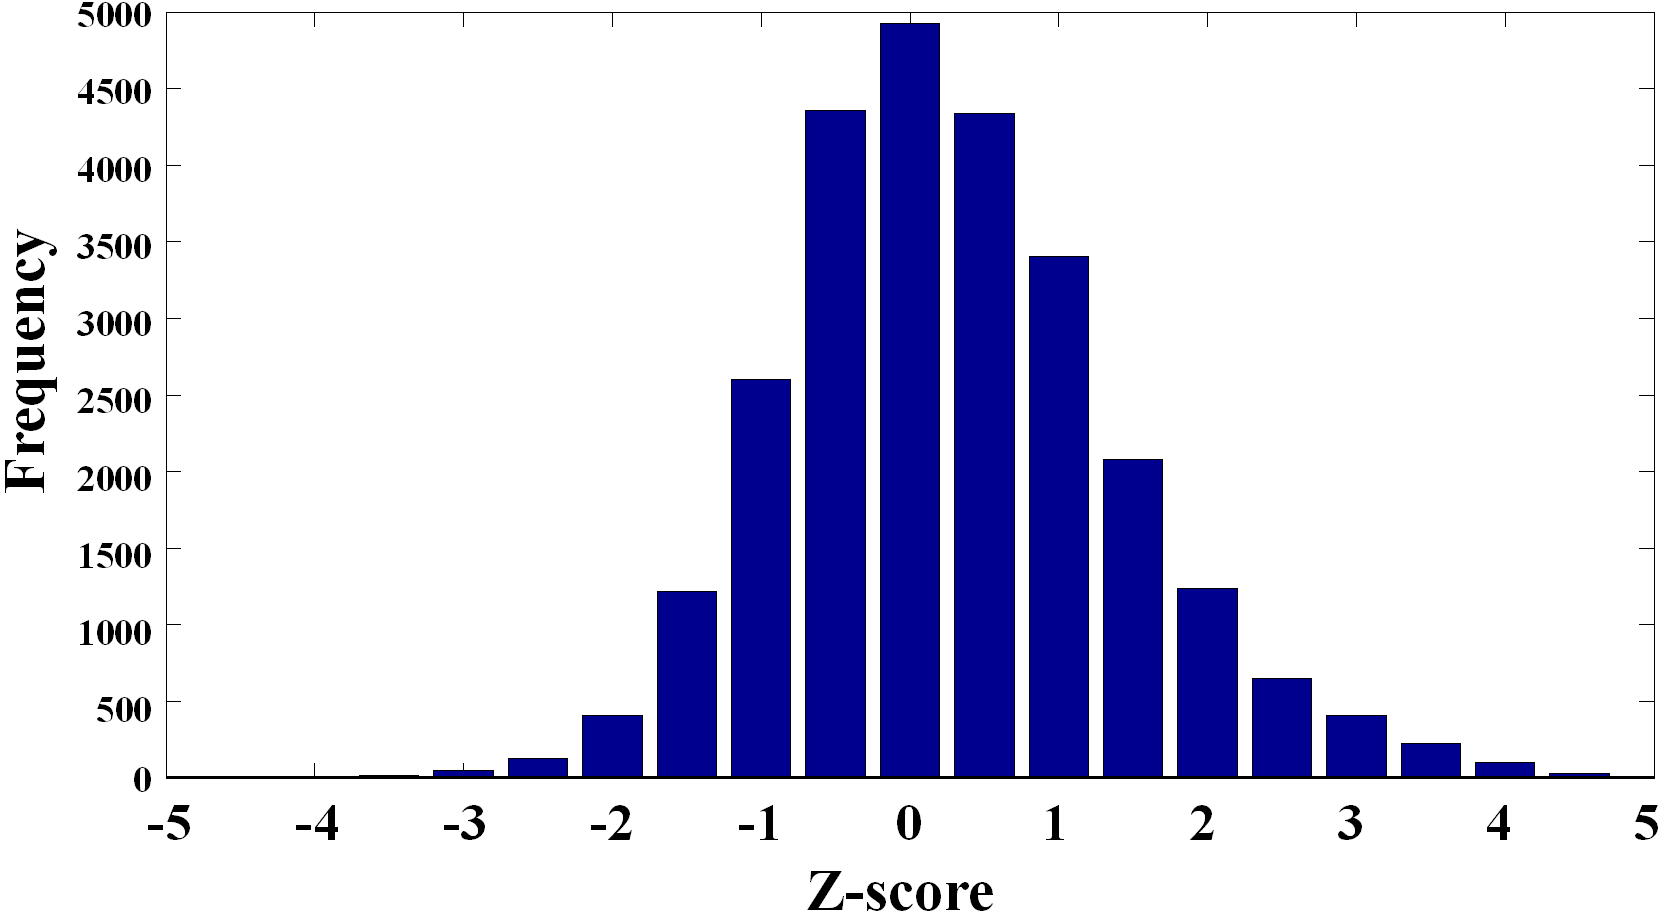
\includegraphics[width=3in] {figures/Z-Score-distribution.png}
		\label{fig:distribution}
	}
	\caption{ Z-score distribution of city Sao Paulo, Brazil from Aug 1, 2012 to January 30, 2014 with time interval of five minutes. }
	\label{fig:zscore-distribution}
\end{figure}
